\chapter{Results}
\begin{toDo}
	\section{Architecture}
	Come accennato nei capitoli precedenti il sistema di analisi delle immagini richiede di confrontare l'opera sconosciuta con quelle note. In particolare l'immagine viene preprocessata rimuovendo elementi inquinanti che non riguardano la grafia, lasciando essenzialmente un'immagine in scala di grigi con in scuro la grafia dell'autore e lo sfondo bianco. Inoltre potrebbe servire che il tratto dell'autore abbia uno spessore specifico rispetto i caratteri impressi e che anche la risoluzione (espressa in \gls{dpi}) sia adatta al dataset.

	\noindent L'immagine così preprocessata sarà quindi sintetizzata, un programma ne estrae tutte le tessere con un size specifico conforme al dataset. In seguito l'immagine sarà confrontata con ogni immagine del dataset (o le più rappresentative per ogni autore).

	\noindent In questo capitolo si effettueranno analisi di ogni passaggio illustrato in questa tesi al fine di vedere come ogni singola componente agisce sulle immagini esaminate. Non solo, si mostreranno anche le analisi effettuate per stabilire specifiche decisioni e parametri usati durante la fase di progettazione.

	\subsection{Implementation}
	L'implementazione del codice ha richiesto notevoli sforzi poiché gran parte dei frame-work richiesti non erano esistenti, inoltre anche le limitazioni della potenza di calcolo e il tempo a disposizione sono state un forte vincolo che ha richiesto la stesura di codice altamente prestante e sofisticato.

	\noindent In generale il progetto ha richiesto largo uso di \gls{Python} e \gls{CUDA}, durante la sua realizzazione si sono usati software specifici per debugging, logging e testing utili per monitorare il corretto funzionamento del software, in particolare si sta parlando di:
	\begin{itemize}
		\item Debugger di \gls{Python} fornito da \gls{VSCode}, \gls{gdb} to debug \gls{cxx} and \gls{CUDA} code
		\item Separate logging of compiled and scripting code, in this way it was possible see in real-time each main calculus and eventually find rapidly some important error and how to fix it
		\item Test library of \gls{Python} to compare high level code and low level code
	\end{itemize}

	\noindent Sono stati usati strumenti di documentazione automatica come \gls{doxygen} e \gls{sphinx} e strumenti di gestione automatica del codice come \gls{github}. Inoltre è stato adottato un robusto sistema di gestione di errori e di sessioni di calcolo, in questo modo da scongiurare di perdere dati preziosi e tempo di calcolo tramite backup (detti "checkpoint").

    \section{Pre processing}
    Mostrare i risultati del pre processing.
    \begin{itemize}
        \item serie di Fourier applicate a griglie sintetiche per dedurre quali sono le frequenze di nostro interesse: griglie dritte e ruotate, griglie chiare e scure, griglie con elementi inquinanti, confronto tra teoria e aspettativa
        \item serie di Fourier applicate a immagini vere, confronto con le immagini sintetiche
        \item mostrare alcuni risultati della pulizia dei quadretti attraverso le varie fasi dell'algoritmo di pulizia
    \end{itemize}
    \section{Synthesis}
    Mostrare una piccola analisi delle sintesi ottenute e della velocità del programma, magari con dettagli implementativi
    \section{Comparison}
   		Mostrare dettagli del clustering a livello esecutivo, come velocità del programma e confronto con l'esecuzione su CPU
    	\subsection{Results}
    		Mostrare dettagli in esecuzione dei vari valori ottenuti dall'algoritmo di comparazione. Quindi concludere con una panoramica dei risultati ottenuti.
\end{toDo}


%\begin{figure}
%	\centering
%	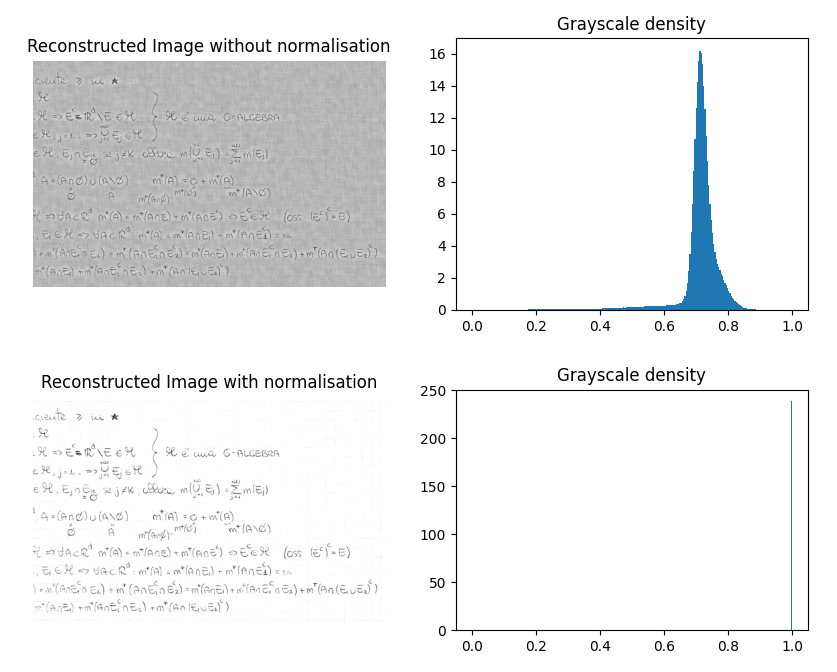
\includegraphics[width=\linewidth]{Figures/first_reconstruct.png}
%	\caption{Come si osserva i grigi si sono molto avvicinati tra loro dopo \gls{fft}, ma è possibile ribilanciare i colori confrontandoli con l'immagine originale.}
%	\label{fig:first_reconstruct}
%\end{figure}
